\chapter{Adjoint method}

In this chapter we are going to discuss the adjoint method: a specific application of reverse mode automatic differentiation which allows to compute efficiently the gradient of a function which depends on many parameters.

To do so we introduce to the possible techniques that allows to compute derivatives using a computer program with particular focus on Automatic Differentiation (AD), highlighting its advantages and its two main implementations.
Subsequently, we will provide a brief overview of design optimization in order to justify the interest in implementing the aforementioned method.
Finally, we conclude the chapter explaining in detail the application of the adjoint method in case of design optimization problems that rely on RBF-FD method for the design analysis stage.

\section{Automatic Differentiation (AD)}

%TODO: Togli questa prima parte, comincia direttamente con il come calcolare le derivate
%Automatic Differentiation (AD) is a family of techniques similar to but more general then backpropagation to efficiently and accurately evaluating derivatives of numeric functions expressed as computer programs. Backpropagation is a well known algorithm used in machine learning and artificial intelligence toolbox being the mainstay for training neural networks. Became popular with the work of Rumelhart in~\cite{Rumelhart:backpropagation_algo} it consists in learning the best set of weights for the network that minimize a certain objective function via an iterative procedure; to do so, for each weights update, a gradient in the weight space has to be computed. The aforementioned gradient is computed by the backpropagation of the sensitivity of the objective function at the output utilizing the chain rule to compute partial derivatives of the objective with respect to each weight. This algorithm is essentially equivalent to the derivative computation via reverse mode AD.

In this section we take 
In general there exists different ways to compute derivatives using a computer program, these are:
\begin{description}
	\item[Manual Differentiation] In this case \emph{analytical} derivatives are computed by hand and then are plugged into standard optimization procedures such as gradient descend. Of course doing so is time consuming and prone to error.
	
	\item[Numerical Differentiation] In this case finite difference methods, as the ones reported in subsection~\ref{subsec:finite_difference_methods}, are used to approximate the derivatives \emph{values}. Easy to implement it has the disadvantage to be inaccurate due to round-off and truncation errors~\cite{LeVeque:FD_book}.

	\item[Symbolic Differentiation] This case addresses the weakness of both manual and numerical differentiation. \emph{Analytical} derivative expressions are automatically obtained by modern computer algebra systems such as Mathematica\footnote{Wolfram Research, Inc.'s proprietary software for technical computing. See~\url{https://www.wolfram.com/mathematica/} for more informations.} or SymPy\footnote{Python open source library for symbolic mathematics. The project can be found at~\url{https://www.sympy.org/en/index.html}.}. Unfortunately, often, the outcomes are plagued with the problem of ``expression swell'' which means that the resulting expressions are large, complex and cryptic. Furthermore it can be applied only to models defined in closed-form.
	
	\item[Automatic Differentiation] This last case refers to a family of techniques that compute derivative \emph{values} (in contrast with symbolic differentiation) by using symbolic rules of differentiation (but keeping track of derivative values as opposed to the resulting expressions) through accumulation of values during code execution. Thanks to this, Automatic Differentiation (AD), can be applied to code involving branches, loops and recursion as opposed to symbolic differentiation~\cite{Baydin:AD_survey}. The mix between symbolic and numerical differentiation gives to these methodologies an hybrid nature.
\end{description}

For the remaining of this section we will explain the details of Automatic Differentiation (AD), to do so we will look at its two (main) implementations:
\begin{itemize}
	\item \emph{forward mode}, also known as tangent linear mode; and
	\item \emph{reverse mode} also known as cotangent linear mode or \emph{adjoint} mode.
\end{itemize}
%\begin{description}
%	\item[Forward mode] also known as tangent linear mode.
%	\item[Reverse mode] also known as cotangent linear mode or \emph{adjoint} mode.
%\end{description}
To explain how each of the two modes works, we show how they are applied to a function $\tilde{f} \colon \R^2 \to \R^2$ defined as:
\begin{equation}
	\label{eqn:example_function_for_AD}
	\tilde{f}(x_1, x_2) = \begin{bmatrix}
					\tilde{f}_1(x_1, x_2)  &  \tilde{f}_2(x_1, x_2)
				  \end{bmatrix}
\end{equation}
with $\tilde{f}_1(x_1, x_2) = x_1 x_2 + \cos x_1$ and $\tilde{f}_2(x_1, x_2) = x_2^3 + \ln x_1 - x_2$.

\smallskip
Before entering into the detail, we notice that every function $f \colon \R^n \to \R^m$ can be rewritten as a computational graph. A computational graph is a direct graph whose nodes correspond to operations and each operation can feed its output into other operations; once the graph is fed with some variables each node become automatically function of those variables. The usual operations considered as nodes are: binary arithmetic operations, the unary sign switch and transcendental functions such as exponential, logarithm and trigonometric functions.
Creating a computational graph for a function becomes easy by indicating with:
\begin{itemize}
	\item $v_{i-n}=x_i$, $i=1, \dots, n$ the input variables;
	\item $v_i$, $i=1, \dots, l$ the intermediate variable;
	\item $y_{m-i}=v_{l-i}$, $i=m-1, \dots, 0$ the output variables.
\end{itemize}
To better identify the relationship between the elementary operations which constitute a function it is helpful creating an \emph{evaluation trace} for the function itself.
Left-hand side of table~\ref{tab:forward_AD_example} and figure~\ref{fig:example_of_computational_graph} contains respectively the evaluation trace and the computational graph for function $\tilde{f}$.

\begin{figure}
\centering
\begin{tikzpicture}
	[circle, inner sep=0pt, minimum size=10mm,
	operation/.style={draw},
	input/.style={draw=none},
	output/.style={draw=none}, -latex, auto, semithick]
	
	
	\node[operation] (v_minus_one) 				   								   {$v_{-1}$};
	\node[operation] (v_zero)	   [below=of v_minus_one, yshift=-20mm] 		   {$v_0$};
	\node[input]	 (x_one)	   [left=of v_minus_one] 						   {$x_1$};
	\node[input]	 (x_two)	   [left=of v_zero] 							   {$x_2$};
	
	\node[operation] (v_one)       [right=of v_minus_one, xshift=5mm, yshift=10mm] {$v_1$};
	\node[operation] (v_two)       [below=of v_one] 							   {$v_2$};
	\node[operation] (v_three)     [below=of v_two] 							   {$v_3$};
	\node[operation] (v_four)      [below=of v_three] 							   {$v_4$};
	
	\node[operation] (v_six)       [right=of v_four, xshift=5mm] 				   {$v_6$};
	
	\node[operation] (v_seven)     [right=of v_six, xshift=5mm, yshift=10mm] 	   {$v_7$};
	\node[operation] (v_five)      [above=of v_seven, yshift=20mm] 			   	   {$v_5$};
	\node[output]	 (f_one)	   [right=of v_five] 							   {$f_1(x_1,x_2)$};
	\node[output]	 (f_two)	   [right=of v_seven] 							   {$f_2(x_1,x_2)$};
	
	
	\draw [->] (x_one)		 to (v_minus_one);
	\draw [->] (x_two)		 to (v_zero);
	\draw [->] (v_minus_one) to (v_one);
	\draw [->] (v_minus_one) to (v_two);
	\draw [->] (v_minus_one) to (v_four);
	\draw [->] (v_zero) 	 to (v_two);
	\draw [->] (v_zero) 	 to (v_three);
	\draw [->] (v_zero) 	 to (v_seven);
	\draw [->] (v_one)		 to (v_five);
	\draw [->] (v_two)		 to (v_five);
	\draw [->] (v_three)	 to (v_six);
	\draw [->] (v_four)	 	 to (v_six);
	\draw [->] (v_six)		 to (v_seven);
	\draw [->] (v_five)		 to (f_one);
	\draw [->] (v_seven)	 to (f_two);
\end{tikzpicture}
\caption{Computational graph of function $\tilde{f}(x_1, x_2) = \Bigl[
		\tilde{f}_1(x_1, x_2) \,\, \tilde{f}_2(x_1, x_2) \Bigr]$. Definitions of intermediate variables $ v_{-1}, \dots, v_7$ can be found in table~\ref{tab:forward_AD_example} or table~\ref{tab:reverse_AD_example}}
\label{fig:example_of_computational_graph}
\end{figure}

\begin{table}
	\centering
	\begin{tabular}{cll}
		\toprule
		\multicolumn{3}{l}{\text{Forward Primal Trace}}  	 \\
		$v_{-1}$ &  $=x_1$ 				  & $=2$  			 \\
		$v_0$	 &  $=x_2$ 				  & $=3$  			 \\
		\midrule
		$v_1$	 &  $=\cos v_{-1}$  	  & $=\cos 2$      	 \\
		$v_2$	 &  $=v_{-1}  v_0$  	  & $=2 \cdot 3$  	 \\
		$v_3$	 &  $=v_0^3$  			  & $=3^3$	  	  	 \\
		$v_4$	 &  $=\ln v_{-1}$  	  	  & $=\ln 2$  	  	 \\
		$v_5$	 &  $=v_2 + v_1 \quad$    & $=6-0.416$   	 \\
		$v_6$	 &  $=v_3 + v_4$  		  & $=27+0.693$  	 \\
		$v_7$	 &  $=v_6 - v_0$  		  & $=27.693-3$  	 \\
		\midrule
		$y_1$	 &  $=v_5$				  & $=5.584$		 \\
		$y_2$	 &  $=v_7$				  & $=24.693$		 \\
		\bottomrule
	\end{tabular}
	%	\begingroup\setlength{\fboxsep}{0pt}
	%	\colorbox{lightgray}{
		\begin{tabular}{cll}
			\toprule
			\multicolumn{3}{l}{\text{Forward Tangent (Derivative) Trace}}  							 \\
			$v'_{-1}$ 		 &  $=x'_1$						  			& $=1$  					 \\
			$v'_0$	  		 &  $=x'_2$ 					  			& $=0$  					 \\
			\midrule
			$v_1'$	  		 &  $=-v_{-1}'\sin v_{-1}$  	  			& $= -1 \cdot \sin 2$      	 \\
			$v_2'$	  		 &  $=v_{-1}'  v_0 + v_{-1}  v_0' \quad$	& $=1 \cdot 3 + 2 \cdot 0$ 	 \\
			$v_3'$	  		 &  $=3  v_o^2  v_0'$  						& $=3 \cdot 2^2 \cdot 0$  	 \\
			$v_4'$	  		 &  $=v_{-1}' / v_{-1}$  			  		& $=1/2$	  	  	 		 \\
			$v_5'$	  		 &  $=v_2' + v_1'$  		  				& $=3 - 0.909$   	 		 \\
			$v_6'$	  		 &  $=v_3' + v_4'$  		  				& $=0+0.5$  	  			 \\
			$v_7'$	  		 &  $=v_6' - v_0'$  		  				& $=0.5 - 0$  				 \\
			\midrule
			$\mathbf{y'_1}$	 &  $\mathbf{=v_5'}$				  		& $\mathbf{=2.091}$			 \\
			$\mathbf{y'_2}$	 &  $\mathbf{=v_7'}$				  		& $\mathbf{=0.5}$			 \\
			\bottomrule
		\end{tabular}
		%	} \endgroup
	\caption{Forward mode AD example to evaluate the derivatives $\frac{\partial y_1}{\partial x_1}$ and $\frac{\partial y_2}{\partial x_1}$ of $\tilde{f}(x_1, x_2)$ at $[x_1, x_2] = [2,3]$. $x_1'$ and $x_2'$ are respectively set to $1$ and $0$ in order to derive only respect $x_1$. On the left is reported the forward evaluation trace, on the right the tangent one}
	\label{tab:forward_AD_example}
\end{table}

Using the aforementioned representations we see that every function ultimately is a composition of elementary operations. This also means that its numerical derivatives can be computed by combining all the numerical derivatives of the constituent operations through the \emph{chain rule}: this, is the main idea of Automatic Differentiation.

%TODO: 1) Talk about automatic label misconception
%Before going ahead we would like to draw reader's attention on the risk of ambiguity that the term ``automatic'' in  AD generate. One might label as AD every technique that allows to compute derivatives without computing them manually (e.g. Symbolic Differentiation), but in technical terms AD is used to indicate only those techniques that compute derivatives through accumulation of values during code execution to generate numerical numerical derivative evaluations rather than derivative expression.


\subsection{Forward mode}
\label{subsec:forward_mode_AD}

In order to compute the derivative of the function $\tilde{f}$, reported in~\eqref{eqn:example_function_for_AD}, respect to $x_1$ we start by considering the evaluation trace on the left-hand side of table~\ref{tab:forward_AD_example} and we associate to each intermediate variable $ v_i$ the derivative:
\[
	v_i' = \frac{\partial v_i}{\partial x_1}
\]
Here the variable with respect to which we differentiate remain the same independently on $i$.
Moving from top to bottom in the forward primal trace the corresponding tangent (derivative) trace, presented on the right-hand side of table~\ref{tab:forward_AD_example}, is generated by applying the chain rule to each encountered operation. After the primals $v_i$ are evaluated, also the corresponding tangents $v_i'$ are, again, from top to bottom, which means that tangent trace can be computed in parallel with the forward trace. This gives us the desired derivatives in the final variables $v_5' = \frac{\partial y_1}{\partial x_1}$ and $v_7' = \frac{\partial y_2}{\partial x_1}$.
%TODO: Cite the fact the output is exact except for floating point appprox

\medskip
Forward mode can also be employed to evaluate the Jacobian of a generic function $f \colon \R^n \to \R^m$ at a point $\vec{x} = \vec{a}$ by performing $n$ distinct forward passes. By setting only one variable $x_i'=1$ and the others to zero we obtain:
\[
	y_j' = \frac{\partial y_j}{\partial x_i}\bigg|_{\vec{x}=\vec{a}} \qquad j=1,\dots,m.
\]
and reiterating for $i=1,\dots,n$, placing the resulting vectors side by side, we eventually obtain the desired Jacobian:
\[
\vec{J}_f =
\left.
\begin{bmatrix}
	\frac{\partial y_1}{\partial x_1} &  \dots  & \frac{\partial y_1}{\partial x_n}  \\
	\vdots							  & \ddots  & \vdots							 \\
	\frac{\partial y_m}{\partial x_n} &  \dots  & \frac{\partial y_m}{\partial x_n}
\end{bmatrix}
\right|_{\vec{x} = \vec{a}}
\]

Furthermore, by properly fine-tuning the values of the variables $x_1', \dots, x_n'$, it is possible to compute efficiently and in a matrix-free way Jacobian-vector products:
\[
\vec{J}_f \vec{r} =
\begin{bmatrix}
	\frac{\partial y_1}{\partial x_1} &  \dots  & \frac{\partial y_1}{\partial x_n}  \\
	\vdots							  & \ddots  & \vdots							 \\
	\frac{\partial y_m}{\partial x_1} &  \dots  & \frac{\partial y_m}{\partial x_n}
\end{bmatrix}
\begin{bmatrix}
	r_1		\\
	\vdots  \\
	r_n
\end{bmatrix}
\]
To accomplish this all that needs to be done is simply initializing $\vec{x}'=\big[x_1', \dots, x_n' \big]$ with $\vec{r}$; this result is particularly important in the evaluation of directional derivatives.
Before moving on, it is crucial to point out that forward mode AD:
\begin{itemize}
	\item for a function $f \colon \R \to \R^m$ allows to evaluate all its derivatives in just one forward pass, regardless of $m$;
	\item for a scalar field $f \colon \R^n \to \R$, the evaluation of its gradient $\nabla f = \Bigl[ \frac{\partial y}{\partial x_1}, \dots, \frac{\partial y}{\partial x_n} \Bigr]$ always require $n$ evaluations (since gradient is nothing more than a Jacobian of size $1 \times n$).
	%TODO: Add note of the factthat that it is not advantageous respect others methods (FD methods also scales linearly??)
\end{itemize}
This means that the here explained implementation of Automatic Differentiation (AD) has a computational cost which scales linearly with the number of function inputs. It is effective during the computation of derivative for cases $f \colon \R^n \to \R^m$ where $n \ll m$; for cases $n \gg m$ \emph{reverse mode} is more beneficial: we will discover why in the next subsection.

%TODO: 1) Aggiungi colore alla tabella di dx
%TODO: 2) Aggiungi descrizione tabelle
%TODO: 3) Aggiungi frecce alle tabelle

\subsection{Reverse mode}
\label{subsec:reverse_mode_AD}

In this case, as opposed to forward mode AD, the derivatives are propagated back from a given output: this means that the underlying mechanism is similar, yet more general, to backpropagation algorithm used in neural networks.
%A demonstration of how it works is presented in table~\ref{tab:reverse_AD_example} where we compute the sensitivities, i.e. of output $y_1 = \tilde{f}_1(x_1, x_2)$ of $\tilde{f}$ respect the inputs $x_1$ and $x_2$.

To do so, different variables, called adjoints, are associated to each variable $v_i$ of the Forward Primal Trace and each of them is defined as:
\[
\overline{v}_i = \frac{\partial y_j}{\partial v_i}
\]
which is nothing more than the sensitivity of the output $y_j$ with respect to changes in $v_i$. It is important for the reader to note that, with this mode, the variable with respect to the derivatives are computed is not fixed as in forward mode AD. An example of reverse mode AD is presented in table~\ref{tab:reverse_AD_example} where we show how to compute the sensitivities of the output $y_1 = \tilde{f}_1(x_1, x_2)$ respect the inputs $x_1$ and $x_2$.

\begin{table}
	\centering
	\begin{tabular}{cll}
		\toprule
		\multicolumn{3}{l}{\text{Forward Primal Trace}}  	 \\
		$v_{-1}$ &  $=x_1$ 				  & $=2$  			 \\
		$v_0$	 &  $=x_2$ 				  & $=3$  			 \\
		\midrule
		$v_1$	 &  $=\cos v_{-1}$  	  & $=\cos 2$      	 \\
		$v_2$	 &  $=v_{-1}  v_0$  	  & $=2 \cdot 3$  	 \\
		$v_3$	 &  $=v_0^3$  			  & $=3^3$	  	  	 \\
		$v_4$	 &  $=\ln v_{-1}$  	  	  & $=\ln 2$  	  	 \\
		$v_5$	 &  $=v_2 + v_1 \quad$    & $=6-0.416$   	 \\
		$v_6$	 &  $=v_3 + v_4$  		  & $=27+0.693$  	 \\
		$v_7$	 &  $=v_6 - v_0$  		  & $=27.693-3$  	 \\
		\midrule
		$y_1$	 &  $=v_5$				  & $=5.584$		 \\
		$y_2$	 &  $=v_7$				  & $=24.693$		 \\
		\bottomrule
	\end{tabular}
	%	\begingroup\setlength{\fboxsep}{0pt}
	%	\colorbox{lightgray}{
		\begin{tabular}{clll}
			\toprule
			\multicolumn{4}{l}{\text{Reverse Adjoint (Derivative) Trace}}  							 \\[2ex]
			$\mathbf{\overline{x}_1}$  &  $\mathbf{ =\frac{\partial y_1}{\partial v_{-1}} \frac{\partial v_{-1}}{\partial x_1} }$  & $\mathbf{=\overline{v}_{-1} \cdot 1 }$  &  $=2.091$  \\[2ex]
			$\mathbf{\overline{x}_2}$  &  $\mathbf{ =\frac{\partial y_1}{\partial v_0} \frac{\partial v_0}{\partial x_2}}$  	   &  $\mathbf{ =\overline{v}_0 \cdot 1 }$   &  $=2$		  \\[2ex]
			
			\midrule
			$\overline{v}_{-1}$  &  $=\frac{\partial y_1}{\partial v_1} \frac{\partial v_1}{\partial v_{-1}} + \frac{\partial y_1}{\partial v_2} \frac{\partial v_2}{\partial v_{-1}} + \frac{\partial y_1}{\partial v_4} \frac{\partial v_4}{\partial v_{-1}}$  &  $=-\overline{v}_1 \sin (v_{-1}) + \overline{v}_2 v_0 + \overline{v}_4/v_{-1}$  &  $=2.091$  \\[2ex]
			$\overline{v}_0$	 &  $=\frac{\partial y_1}{\partial v_2} \frac{\partial v_2}{\partial v_0} + \frac{\partial y_1}{\partial v_3} \frac{\partial v_3}{\partial v_0}$  & $=\overline{v}_2 v_{-1} + 3 \overline{v}_3 v_0^2$  &  $=2$  \\[2ex]
			$\overline{v}_1$	 &  $=\frac{\partial y_1}{\partial v_5} \frac{\partial v_5}{\partial v_1}$  &  $=\overline{v}_5 \cdot 1$  &  $=1$  \\[2ex]
			$\overline{v}_2$	 &  $=\frac{\partial y_1}{\partial v_5} \frac{\partial v_5}{\partial v_2}$  &  $=\overline{v}_5 \cdot 1$  &  $=1$  \\[2ex]
			$\overline{v}_3$	 &  $=\frac{\partial y_1}{\partial v_6} \frac{\partial v_6}{\partial v_3}$  &  $=\overline{v}_6 \cdot 1$  &  $=0$  \\[2ex]
			$\overline{v}_4$	 &  $=\frac{\partial y_1}{\partial v_6} \frac{\partial v_6}{\partial v_4}$  &  $=\overline{v}_6 \cdot 1$  &  $=0$  \\[2ex]
			$\overline{v}_6$	 &  $=\frac{\partial y_1}{\partial v_7} \frac{\partial v_7}{\partial v_6}$  &  $=\overline{v}_7 \cdot 1$  &  $=0$  \\[2ex]
			
			\midrule
			$\overline{v}_5$  &  $=\overline{y}_1$	&  &  $=1$	\\
			$\overline{v}_7$  &  $=\overline{y}_2$  &  &  $=0$	\\
			\bottomrule
		\end{tabular}
		%	} \endgroup
	\caption {Reverse mode AD example with $[y_1, y_2] = \tilde{f}(x_1, x_2)$ evaluated at $[x_1, x_2] = [2,3]$. First, primal trace is evaluated (table above) and then adjoint variables are computed, from the  bottom up, in a second phase (table below). The initialization $\overline{v}_5 = \frac{\partial y_1}{\partial v_5} = \frac{\partial y_1}{\partial y_1} = \overline{y}_1 = 1$ and $\overline{v}_7 = \frac{\partial y_1}{\partial v_7} = \frac{\partial y_1}{\partial y_2} = \overline{y}_2 = 0$ is such that it allows the sensitivities to be calculated with respect the fist output}
	%	\caption{Reverse mode AD example to evaluate the derivatives $\frac{\partial y_1}{\partial x_1}$ and $\frac{\partial y_1}{\partial x_2}$ of $\tilde{f}(x_1, x_2)$ at $[x_1, x_2] = [2,3]$. $y_1'$ and $y_2'$ are respectively set to $1$ and $0$ in order to obtain the sensitivities respect $y_1$. Above is reported the forward evaluation trace, below the adjoint one}
	\label{tab:reverse_AD_example}
\end{table}

\clearpage

Since typical usage of chain rule is forward derivatives propagation, reverse mode AD might appear confusing at first sight; to make it clearer we show how the chain rule can be used to back-propagating derivatives in order to compute the contribution $\overline{v}_0$ of the change in variable $v_0$ to the change in the output $y_1$. From figure~\ref{fig:example_of_computational_graph} can be seen that the only way variable $v_0$ can affect $y_1$ is through affecting $v_2$ and $v_3$, so its contribution to the change in $y_1$ can be computed using the chain rule as follow:
\begin{equation}
	\frac{\partial y_1}{\partial v_0} = \frac{\partial y_1}{\partial v_2} \frac{\partial v_2}{\partial v_0} + \frac{\partial y_1}{\partial v_3} \frac{\partial v_3}{\partial v_0}
\end{equation}
which can be rewritten in
\begin{equation}
	\begin{split}
		\frac{\partial y_1}{\partial v_0} & = \overline{v}_2 \frac{\partial v_2}{\partial v_0} + \overline{v}_3 \frac{\partial v_3}{\partial v_0}  \\[2ex]
										  & = \overline{v}_2 v_{-1} + 3 \overline{v}_3 v_0^2
	\end{split}
\end{equation}
where quantities $\overline{v}_2$ and $\overline{v}_3$ are known from previous passages and derivatives $\frac{\partial v_2}{\partial v_0}$, $\frac{\partial v_3}{\partial v_0}$, can be easily computed by evaluating the result of symbolic differentiation of the elementary operations on the primals $v_i$.

\medskip
In light of the previous example, it is clear that, to compute derivatives, primals $v_i$ must be known along their dependencies within the computational graph. To do so two phases are required:
\begin{itemize}
	\item A \emph{forward step} where variables $v_i$ are populated and their dependencies recorded;
	\item A \emph{reverse step} where adjoints $\overline{v}_i$ are evaluated from outputs to inputs using values obtained in the first step.
\end{itemize}
We remark that once the backward pass is completed we get \emph{all} the sensitivities $\frac{\partial y_j}{\partial x_1}, \dots, \frac{\partial y_j}{\partial x_n}$ in one single pass; this means that for scalar fields $f \colon \R^n \to \R$ the computation of the gradient $\nabla f$ require only one application of reverse mode as opposed to the $n$ passes required in case of forward mode. Nevertheless, this advantage comes at the cost of increased memory requirements which grows proportionally (in the worst case) to the number of operations in the evaluated function~\cite{Baydin:AD_survey}.

Generalizing the reasoning to functions $f \colon \R^n \to \R^m$, similarly to how it was done in previous section, we can conclude that reverse mode AD can also be used to evaluate Jacobians at a point; in particular, since each pass of reverse AD allows to compute one row of the Jacobian, its usage is advantageous when $m \ll n$ .
With regard to products between Jacobain and vector, reverse AD allows to compute efficiently vector-Jacobian products of type:
\begin{equation}
	\vec{r}^T \vec{J}_f =
	\begin{bmatrix}
		r_1 	& \dots  & r_m
	\end{bmatrix}
	\begin{bmatrix}
		\frac{\partial y_1}{\partial x_1} &  \dots  & \frac{\partial y_1}{\partial x_n}  \\
		\vdots							  & \ddots  & \vdots							 \\
		\frac{\partial y_m}{\partial x_1} &  \dots  & \frac{\partial y_m}{\partial x_n}
	\end{bmatrix}
\end{equation}
by initializing $\vec{\overline{y}}=\big[\overline{y}_1, \dots, \overline{y}_m \big]$ with $\vec{r}$.


%TODO: Valuta la notazione $\vec{\overline{y}}$ che è un po' ambigua nel caso in cui cambi output da differenziare
%TODO: Cita più spesso AD survey 


\section{Application to design optimization}
\label{sec:application_to_design_opt}

Design optimization is a topic that spans multiple disciplines, examples include, but are not limited to: wing configuration in aerospace, structural design in civil engineering, circuit design in electrical engineering, mechanism design in mechanical engineering and neural networks sizing and arches weighting in computer science.
An example of the results that can be achieved through design optimization is shown in figure~\ref{fig:wing_opt}.

\begin{figure}
	\centering
	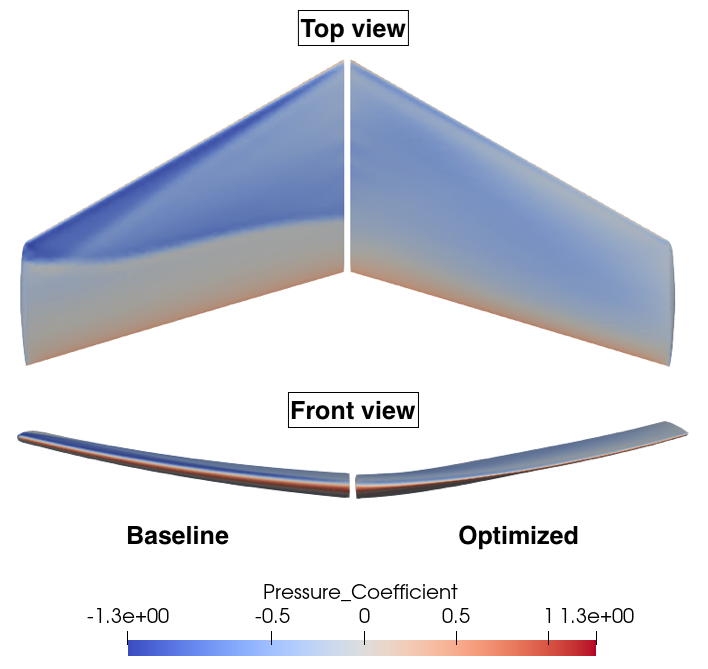
\includegraphics[width=.5\textwidth]{img/wing_opt.png}
	\caption{Example of design optimization: baseline and final design of ONERA M6 wing is shown. It can be seen how the relative pressure exerted by the air on the wing has been minimized. Figure taken from~\cite{Bombardieri:paper_of_wing_opt_image}}
	\label{fig:wing_opt}
\end{figure}

From a formal point of view it is the process of finding the best design parameters $\vec{l} = [l_1, \dots, l_N]$ that satisfy project requirements~\cite{Matlab:design_opt}. Requirements and objectives, which are usually multiple and conflicting, are typically expressed in the form of a scalar function $J \colon \R^M\times\R^N \to \R$ named \emph{cost} or \emph{objective function}. $J$ depends on the state $\vec{u} \in \R^M$ of the problem at hand and on the design parameters $\vec{l} \in \R^N$; $\vec{u}$ is generally found as solution of a system of linear equations $\vec{Au} = \vec{b}$, which arise from the imposition of the constraints of the problem, where $\vec{A} \in \R^{M \times M}$ and $\vec{b} \in \R^M$ depends on some way on $\vec{l}$. In figure~\ref{fig:design_opt_scheme} can be found a scheme of the whole process.

%This type of process is of interest since it is encountered in the most diverse fields, from computer science, where for example the proper weights of a neural network has to be found in order to minimize the error between its predicted and the desired output respect a given set of inputs, to mechanical engineering where, for example, one may want to modify the shape of an heat sink to maximize the amount of the heat transferred to the environment.

\begin{figure}
	\centering
	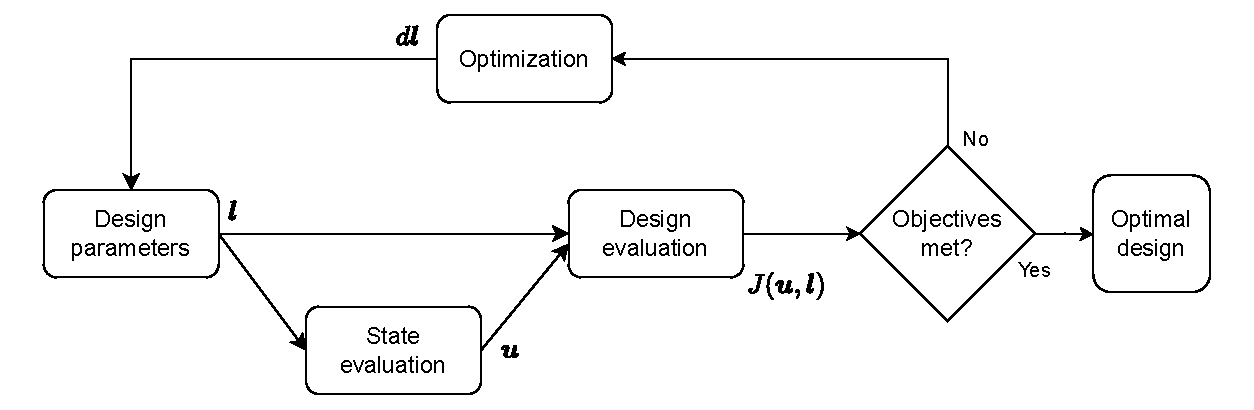
\includegraphics[width=\textwidth]{img/design_opt_scheme.pdf}
	\caption{Scheme of a design optimization process. From an initial design defined by a set of parameters $\vec{l}$ the associated state $\vec{u}$ is derived. The state in conjunction with the parameters are then used to evaluate the design through a function $J$. If the objectives are met the design is kept otherwise the whole procedure is repeated with a new set of parameters obtained by modifying the previous ones by a quantity $\Delta\vec{l}$} 
	\label{fig:design_opt_scheme}
\end{figure}

To find the best parameters for a given project a variety of iterative approaches can be pursued during the optimization phase:
\begin{description}
	\item[Manual approach] where each parameter $l_1, \dots, l_N$ is adjusted one at a time. Unfortunately doing so tends to leads to suboptimal results;
	\item[Brute-force approach] where all possible combinations of design parameters are evaluated. However, this is time-expensive and for large-scale projects, where parameters can be hundreds, thousands, or even more, optimal parameters may not be found in reasonable time-frames;
	\item[Gradient approach] where the gradient $\frac{dJ}{d\vec{l}}$ permits both to update all the parameters $l_1, \dots, l_N$ at the same time and to disregard most of the parameter values that are sub-optimal by considering only those suggested by its direction.
\end{description}
For the effectiveness of the last mentioned approach, is crucial to ensure an efficient computation of the gradient $\frac{dJ}{d\vec{l}}$ which must require as few steps as possible and be efficient even for problems involving huge number of design parameters. To meet these requirements Automatic Differentiation (AD) in its reverse-mode declination is necessary.
%TODO: adjust the end of the "paragraph"

\bigskip
Given its advantages in design optimization we have learned that using the gradient is a good course of action. To directly evaluate $\frac{dJ}{d\vec{l}}$, in case of a particular set of design parameters defined by $\vec{l}$ at a given state $\vec{u}$, we would compute:
\begin{equation}
	\label{eqn:generic_gradient_design_opt}
	\frac{dJ}{d\vec{l}}^T = \frac{\partial J}{\partial \vec{u}}^T \frac{d\vec{u}}{d\vec{l}} + \frac{\partial J}{\partial \vec{l}}^T
\end{equation}
%TODO: Valuta di precisare la notazione da qualce parte invece di metterla in mezzo al documento
where notations $\frac{d}{dx}$ and $\frac{\partial}{\partial x}$ indicate the total and the partial derivatives respect the variable $x$ respectively.
Terms $\frac{\partial J}{\partial \vec{u}}$ and $\frac{\partial J}{\partial \vec{l}}$ can be efficiently obtained by means of reverse-mode AD, as explained in subsection~\vref{:reverse_mode_AD}, since $J$ is known analytically. The matrix $\frac{d\vec{u}}{d\vec{l}}$, on the other hand, require more careful considerations.

Differentiating the problem constraints $\vec{Au} = \vec{b}$ with respect to the parameters $\vec{l}$ gives:
\begin{equation}
	\frac{d\vec{A}}{d\vec{l}} \vec{u} + \vec{A} \frac{d\vec{u}}{d\vec{l}} = \frac{d\vec{b}}{d\vec{l}}
\end{equation}
which allows to obtain the sought term $\frac{d\vec{u}}{d\vec{l}}$ as:
\begin{equation}
	\label{eqn:state_sensitivity_respect_single_param}
	\frac{d\vec{u}}{d\vec{l}} = \vec{A}^{-1} \left( \frac{d\vec{b}}{d\vec{l}} - \frac{d\vec{A}}{d\vec{l}}\vec{u} \right)
\end{equation}
We notice that $\frac{d\vec{u}}{d\vec{l}}$ is a matrix of size $M \times N$ whose $j$-th column represent the sensitivity of the state $\vec{u}$ respect to the parameter $l_j$. 
In practice it is populated column-wise by solving equation~\eqref{eqn:state_sensitivity_respect_single_param} $N$ times when the derivative is taken with respect the $j$-th design parameter $l_j$ rather than $\vec{l}$: this gives its $j$-th column. In this process $\frac{d\vec{b}}{d\vec{l}}$ and $\frac{d\vec{A}}{d\vec{l}}$ terms can be simply obtained using AD, if $\vec{b}$ and $\vec{A}$ are known analytically, and once $\frac{d\vec{u}}{d\vec{l}}$ is computed it can be substituted in equation~\eqref{eqn:generic_gradient_design_opt} to obtain the gradient which symbolically reads as:
\begin{equation}
	\label{eqn:generic_gradient_design_opt_naive}
	\frac{dJ}{d\vec{l}} = \frac{\partial J}{\partial \vec{u}}^T \left[ \vec{A}^{-1} \left( \frac{d\vec{b}}{d\vec{l}} - \frac{d\vec{A}}{d\vec{l}}\vec{u} \right) \right]  + \frac{\partial J}{\partial \vec{l}}^T
\end{equation}

However the computational costs of this naive procedure scales linearly with the number of the design parameters $N$, since $N$ solutions of liner systems are required in order to construct $\frac{d\vec{u}}{d\vec{l}}$. We finally remark that each of these inversions has the same computational cost of solving $\vec{A} \vec{u}= \vec{b}$ for $\vec{u}$ and if the solution represent the output of a particularly time consuming computation, as a CFD simulation is an example of, this is particularly penalizing. A more efficient gradient computation is therefore required.

\smallskip
To do so we can employ the \emph{adjoint method} which simply consist of a smarter bracketing of the equation which gives the gradient. In fact is possible to rewrite~\eqref{eqn:generic_gradient_design_opt_naive} as:
\begin{equation}
	\begin{aligned}
		\frac{dJ}{d\vec{l}} & = \left[ \frac{\partial J}{\partial \vec{u}}^T \vec{A}^{-1} \right] \left( \frac{d\vec{b}}{d\vec{l}} - \frac{d\vec{A}}{d\vec{l}}\vec{u} \right) + \frac{\partial J}{\partial \vec{l}}^T  \\[2ex]
							& = \vec{\lambda}^T \left( \frac{d\vec{b}}{d\vec{l}} - \frac{d\vec{A}}{d\vec{l}}\vec{u} \right) + \frac{\partial J}{\partial \vec{l}}^T
	\end{aligned}
\end{equation}
where the vector $\vec{\lambda} \in \R^L$, whose elements are called \emph{adjoint variables}, can be found by solving:
\begin{equation}
	\label{eqn:generic_adjoint_system_design_opt}
	\vec{A}^T \vec{\lambda} = \frac{\partial J}{\partial \vec{u}}
\end{equation}

By doing so is possible to solve the system in equation~\eqref{eqn:generic_adjoint_system_design_opt}, which is called \emph{adjoint problem}, only \emph{once} independently on the number $N$ of design parameters for each gradient computation: this significantly reduces the computational burden of the whole optimization process. Bear in mind that the adjoint problem has the same size as the problem defined by the constraints $\vec{A} \vec{u} = \vec{b}$ and the computational cost for their solution is the same.

\bigskip
At this point it is worth noting that the adjoint method explained above is just a particular application of reverse mode AD. To make the connections between the two methods clearer we note that the first computation of the  objective function's gradient, presented in equation~\eqref{eqn:generic_gradient_design_opt}, contains the following vector-Jacobian product:
\begin{equation}
	\label{eqn:vJp_design_opt}
	\frac{\partial J}{\partial \vec{u}}^T \frac{d\vec{u}}{d\vec{l}}
\end{equation}
where $\frac{\partial J}{\partial \vec{u}}^T \in \R^M$ is the vector that multiply $\frac{d\vec{u}}{d\vec{l}} \in \R^{M \times N}$, the Jacobian of the state $\vec{u}$ respect the design parameters $\vec{l}$.
From subsection~\vref{subsec:reverse_mode_AD} we known that AD allows to compute the resulting vector without explicitly computing the Jacobian $\frac{d\vec{u}}{d\vec{l}}$. But this is precisely what the adjoint method does through equations~(\ref{eqn:generic_gradient_design_opt} -~\ref{eqn:generic_adjoint_system_design_opt}) by first applying the chain rule to the leftmost term in the gradient formula and then parenthesizing the result in order to make the number of inversions of the matrix $\vec{A}$ independent on the number of parameters.
The result of the whole process is then summarized by:
\begin{equation}
	\label{eqn:resulting_term_adjoint_method}
	\vec{\lambda}^T \left( \frac{d\vec{b}}{d\vec{l}} - \frac{d\vec{A}}{d\vec{l}}\vec{u} \right)
\end{equation}
where $\vec{\lambda}$ solves equation~\eqref{eqn:generic_adjoint_system_design_opt} and the Jacobian $\frac{d\vec{u}}{d\vec{l}}$ is no more present. Furthermore the two-steps process of the reverse mode AD for the gradient computation is still there even in the adjoint method:
\begin{itemize}
	\item the forward pass, used for the computation of variables $v_i$ in table~\ref{tab:reverse_AD_example}, now is the single solution of the system $\vec{A}\vec{u}=\vec{b}$ in order to find the state $\vec{u}$ used in term~\eqref{eqn:resulting_term_adjoint_method};
	\item the reverse pass, done in order to obtain the adjoint variables $\overline{v}_i$ in table~\ref{tab:reverse_AD_example}, is now equivalent to the solution of $\vec{A}^T \vec{\lambda} = \frac{\partial J}{\partial \vec{u}}$ (we would like to reiterate again that reverse and forward pass has the \emph{same} computational complexity). 
\end{itemize}

After this concise overview of the adjoint method applied to generic design optimization problems, we now proceed to the next section where we examine in more detail its application to those problems which state $\vec{u}$ is obtained solving a Partial Differential Equation by means of RBF-FD methods.



\section{Application to RBF-FD}

In section~\ref{sec:RBF-FD} we have seen how the RBF-FD solver for Partial Differential Equations (PDEs) is implemented. Computational Fluid Dynamics (CFD), where PDEs are employed to model fluid flow and heat transfer problems, is one of the main areas where the application of the RBF-FD method could bring great benefits.
CFD is one of the main engineering application where design optimization problems arises almost naturally. However the computational cost of the optimization in the analysis hase is very high it would be of interest apply the adjoint method in those problema

%In section~\ref{sec:RBF-FD} we have seen how the RBF-FD solver for Partial Differential Equations (PDEs) is implemented. Computational Fluid Dynamics (CFD), where PDEs involve fluid flows and heat transfers, is one of the main areas of its application. In all these cases design optimization problems arises almost naturally: regarding heat transfers we have already mentioned the heath sink case where heath exchanged with the environment should be maximized, as to fluid flows a typical example is to find the best shape for the wings of an aircraft in order to maximize its lift and/or minimize its drag.

Once a generic description for the design optimization problem has been written it has to be translated into a mathematical statement in order to solve it through an optimization algorithm. To do so the following items are used for a correct formulation:
\begin{itemize}
	\item \emph{Design variables} represented by a vector $\vec{l} = \left[ l_1, \dots, l_L \right] \in \R^L$. We consider only continuous variables since they control the shape objects which are allowed to vary continuously in the space;
	
	\item \emph{Objective function} indicated with $J \colon \R^{N_I}\times\R^L \to \R$. It is a scalar function that yields a quantity used to determines if one design is better than another. It is an explicit function of the state $\vec{u}_I$ of the problem, which is obtained from the RBF-FD solver, and the design parameters $\vec{l}$. Its choice is crucial: it has to represent the real goal of the whole optimization. A poor choice would lead to a mathematical optimum which does not match with the engineering optimum;
	\item \emph{Constraints} represented by the RBF-FD governing equations: these are reported in equation~\eqref{eqn:discretized_version_of_PDE_using_RBF-FD} in subsection~\ref{subsec:RBF-FD_formulation}. We reiterate them here, in a more compact form, since they will be used extensively throughout the rest of this section:
	\begin{equation}
		\label{eqn:compact_discretized_PDE}
		\vec{C}_I \vec{u}_I + \vec{C}_B \vec{u}_B = \vec{f}
	\end{equation}
	where we have used the following notation: $\vec{u}_I = \left[ u(\vec{x}_1), \dots u(\vec{x}_{N_I}) \right]$, $\vec{u}_B = \left[ g(\vec{x}_{N_I+1}), \dots, g(\vec{x}_N) \right]$ and $\vec{f} = \left[ f(\vec{x}_1), \dots, f(\vec{x}_{N_I}) \right]$, recalling that $N$ is the number of RBF-FD nodes scattered throughout the physical domain $\Omega\cup\partial\Omega$ of the system wich is represented by the volume of the object. The first $N_I$ nodes are contained within it, the remaining ones are placed on its surface.
	Before proceeding is worth noting that, in general, matrices $\vec{C}_I$ and $\vec{C}_B$, and vectors $\vec{f}$ and $\vec{u}_B$ depend on design variables $\vec{l}$. Therefore the solution $\vec{u}_I$ will also be a function (indirectly through constraint~\eqref{eqn:compact_discretized_PDE}) of design variables.
\end{itemize}
Therefore the resulting optimization problem can be written as:
\begin{equation}
	\label{eqn:RBF-FD_opt_problem}
	\begin{aligned}
		\text{minimize} & \quad J(\vec{u}_I, \vec{l})								\\
		\text{by varying} & \quad \vec{u}_I											\\
						& \quad \vec{l} 											\\
		\text{subject to} & \quad \vec{C}_I \vec{u}_I + \vec{C}_B \vec{u}_B = \vec{f}					
	\end{aligned}
\end{equation}
which optimum is found through the gradient approach explained in section~\ref{sec:application_to_design_opt}. In general with a similar formulation can be solved also problems which require the maximization of the objective function since $\max \left[ J(\vec{u}_I, \vec{l}) \right] = - \min \left[ - J(\vec{u}_I, \vec{l}) \right]$. Finally we remark that the variables that can be modified at each optimization cycle are only the design variables $\vec{l}$ since the result of CFD simulation $\vec{u}_I$ is fully determined from constraints~\eqref{eqn:compact_discretized_PDE};

In the two following subsections we will explain how the gradient $\frac{dJ}{d\vec{l}}$ can be computed efficiently by means of the adjoint method for the optimization problem~\eqref{eqn:RBF-FD_opt_problem} in case of one and three-dimensional objects.


\subsection{1D}
\label{subsec:adjoint_method_RBF-FD_1D}

In this case we consider a general cost function $J \colon \R^{N_I \times L} \to \R$. Thanks to this generality its sensitivities respect the design parameters are given by the same exact formula used in general design optimization problems:
\begin{equation}
	\label{eqn:gradient_1st_step_1D_RBF-FD}
	\frac{dJ}{d\vec{l}}^T = \frac{\partial J}{\partial \vec{u}_I}^T \frac{d\vec{u}_I}{d\vec{l}} + \frac{\partial J}{\partial \vec{l}}^T
\end{equation}
Once more, what is now lacking is the term $\frac{d\vec{u}_I}{d\vec{l}}$. The sensitivities of the state respect the parameters can be computed by differentiating equation~\eqref{eqn:compact_discretized_PDE} which gives:
\begin{equation}
	\frac{d\vec{C}_I}{d\vec{l}} \vec{u}_I + \vec{C}_I \frac{d\vec{u}_I}{d\vec{l}} + \frac{d\vec{C}_B}{d\vec{l}} \vec{u}_B + \vec{C}_B \frac{d\vec{u}_B}{d\vec{l}} =
	\frac{d\vec{f}}{d\vec{l}}
\end{equation} 
Before proceeding a note on the matrix $\frac{d\vec{u}_B}{d\vec{l}}$ could be useful: one might think that it should not be present since values in $\vec{u}_B$ are fixed from boundary conditions of problem~\eqref{eqn:boundary_value_problem} (i.e. they are not dependent on the design parameters).
Nevertheless the previous statement does not hold in general since the values of $\vec{u}_B$ could directly depend on the design variables (as an example one may think of Dirichlet Boundary Conditions (BCs) defined by $u(\vec{x})=g(\vec{x}, \vec{l})$) or indirectly depend on them through the problem geometry (e.g. Neumann or Robin BCs).

Once $\frac{d\vec{u}_I}{d\vec{l}}$ is isolated from the previous equation it can be plugged in~\eqref{eqn:gradient_1st_step_1D_RBF-FD} which in turns become:
\begin{equation}
\begin{aligned}
	\frac{dJ}{d\vec{l}}^T & = \frac{\partial J}{\partial \vec{u}_I}^T \biggl[ \vec{C}_I^{-1} \biggl( \frac{d\vec{f}}{d\vec{l}} - \frac{d\vec{C}_I}{d\vec{l}} \vec{u}_I - \frac{d\vec{C}_B}{d\vec{l}} \vec{u}_B - \vec{C}_B \frac{d\vec{u}_B}{d\vec{l}} \biggr) \biggr] + \frac{\partial J}{\partial \vec{l}}^T  \\[2ex]
						  & = \frac{\partial J}{\partial \vec{u}_I}^T \biggl[ \vec{C}_I^{-1} \biggl( \frac{d\vec{f}}{d\vec{l}} - \frac{d\vec{C}}{d\vec{l}} \vec{u} - \vec{C}_B \frac{d\vec{u}_B}{d\vec{l}} \biggr) \biggr] + \frac{\partial J}{\partial \vec{l}}^T
\end{aligned}
\end{equation}
where $\frac{d\vec{C}}{d\vec{l}} \in \R^{N_I \times N}$ is the matrix resulting from the concatenation of the rows of $\frac{d\vec{C}_I}{d\vec{l}} \in \R^{N_I \times N_I}$ and $\frac{d\vec{C}_B}{d\vec{l}} \in \R^{N_B \times N_B}$, and $\vec{u} \in \R^{N}$ is the vector given by the concatenation of the elements of $\vec{u}_I \in \R^{N_I}$ and $\vec{u}_B \in \R^{N_B}$.
Now the adjoint method can be employed in order to avoid performing the inversion of matrix $\vec{C}_I$ once for each parameter in $\vec{l}$, yielding:
\begin{equation}
	\frac{dJ}{d\vec{l}}^T =  \vec{\lambda}_1^T \biggl( \frac{d\vec{f}}{d\vec{l}} - \frac{d\vec{C}}{d\vec{l}} \vec{u} - \vec{C}_B \frac{d\vec{u}_B}{d\vec{l}} \biggr) + \frac{\partial J}{\partial \vec{l}}^T  \\
\end{equation}
where $\vec{\lambda}_1$ is found by solving \emph{once}:
\begin{equation}
	\vec{C}_I^T \vec{\lambda}_1 = \frac{\partial J}{\partial \vec{u}_I}
\end{equation}
The unknown terms involving derivatives computation on the right-hand side can be computed easily through AD except for $\frac{d\vec{C}}{d\vec{l}} \vec{u}$. This terms deserves more attentions since requires the differentiation of the global matrix $\vec{C}$ which is obtained by solving $N_I$ local systems, each associated with a different stencil $\mathcal{X}_i$.

\medskip
%Taking a moment to consider the matrix $\frac{d\vec{C}}{d\vec{l}} \vec{u} \in \R^{N \times L}$ we can note that is obtained from a product between a rank-3 tensor 
In order to examine it more closely we can define a matrix $\vec{Q} \in \R^{N_I \times L}$ as follows:
\begin{equation}
	\label{eqn:Q_matrix_definition}
	\vec{Q} = \frac{d\vec{C}}{d\vec{l}} \vec{u}
\end{equation}
whose elements $q_{i,j}$ are given by:
\begin{equation}
	\label{eqn:Q_elements}
	q_{i,j} = \frac{d\vec{C}_{[i,:]}}{dl_j} \vec{u}
\end{equation}
where notation $\vec{C}_{[i,:]}$ is used to indicate the $i$-th row of the matrix $\vec{C}$.
To obtain $\frac{d\vec{C}}{d\vec{l}} \vec{u}$ is thus sufficient to compute each element of $\vec{Q}$ through equation~\eqref{eqn:Q_elements}. However, before doing so, it is worth rewriting the equation for $q_{i,j}$ more explicitly.

Recall that elements that make up the $i$-th row of $\vec{C}$ are found by solving the local system~\eqref{eqn:row_of_C_system}:
\begin{equation}
	\label{eqn:local_RBF-FD_system_adjoint_1D}
	\vec{M}_{BC}^T
	\begin{bmatrix}
		\vec{c}_I(\vec{x}_i)  \\
		\vec{c}_B(\vec{x}_i)  \\
		\vec{c}_p(\vec{x}_i)
	\end{bmatrix} = 
	\begin{bmatrix}
		\mathcal{L} \vec{\Phi}(\vec{x}_i, \mathcal{X}_{i,I})  \\
		\mathcal{L} \vec{p}(\vec{x}_i)
	\end{bmatrix}
\end{equation}
in case of RBF-FD method, or the local system~\eqref{eqn:row_of_C_system_in_RBF-HFD}:
\begin{equation}
	\label{eqn:adjoint_method_row_of_C_system_in_RBF-HFD}
	\vec{M}_{BC}^T
	\begin{bmatrix}
		\vec{c}_I(\vec{x}_i)  \\
		\vec{c}_B(\vec{x}_i)  \\
		\vec{c}_p(\vec{x}_i)
	\end{bmatrix} = 
	\begin{bmatrix}
		\mathcal{L}_1 \vec{\Phi}(\vec{x}_i, \mathcal{X}_{i,I})  			  \\
		\mathcal{L}_1 \mathcal{B}_2 \vec{\Phi}(\vec{x}_i, \mathcal{X}_{i,B})  \\
		\mathcal{L} \vec{p}(\vec{x}_i)
	\end{bmatrix}
\end{equation}
in case of RBF-HFD method. The key aspect that both cases share is that the aforementioned equations arises from the information contained in a single stencil $\mathcal{X}_i$ and, as explained in subsection~\ref{subsec:RBF-FD_formulation}, only the first $m$ elements of $\vec{c}(\vec{x}_i) = \bigl[ \vec{c}_I(\vec{x}_i), \vec{c}_B(\vec{x}_i), \vec{c}_p(\vec{x}_i) \bigr]$ form the $i$-th row of $\vec{C}$. 
Furthermore, since $m \ll N$, row $\vec{C}_{[i,:]}$ is sparse; which in turns implies that not all the elements of $\vec{u}$ are involved in the computation of $q_{i,j}$.

By letting $\vec{\tilde{u}}_i \in \R^m$ the vector composed by the components of $\vec{u}$ associated to the non zero elements of $\vec{C}_{[i,:]}$, we can rewrite the elements of $\vec{Q}$ reported in~\eqref{eqn:Q_elements} as:
\begin{equation}
	\label{eqn:Q_elements_rewritten}
	q_{i,j} =
	\frac{d\vec{c}(\vec{x}_i)^T}{dl_j}
	\begin{bmatrix}
		\vec{\tilde{u}}_i  \\
		\vec{0}
	\end{bmatrix}
\end{equation}
where the zero-vector concatenated to $\vec{\tilde{u}}_i$ has the same length of $\vec{c}_p(\vec{x}_i)$.
If we now differentiate equation~\eqref{eqn:adjoint_method_row_of_C_system_in_RBF-HFD} respect the $j$-th design parameter, we obtain:
\begin{equation}
	\frac{d \vec{M}_{BC}^T}{d l_j} \vec{c}(\vec{x}_i) + \vec{M}_{BC}^T \frac{d \vec{c}(\vec{x}_i)}{d l_j} = \frac{d \vec{h}}{d l_j}
\end{equation}
where the vector $\vec{h} \in \R^{m+M}$ is used as a shorthand for the vector present on the right-hand side of equation~\eqref{eqn:adjoint_method_row_of_C_system_in_RBF-HFD}. Now from the last equation we can isolate:
\begin{equation}
	\frac{d \vec{c}(\vec{x}_i)^T}{dl_j} = \left( \frac{d \vec{h}}{d l_j} - \frac{d \vec{M}_{BC}^T}{d l_j} \vec{c}(\vec{x}_i) \right)^T \vec{M}_{BC}^{-1}
\end{equation}
which once plugged in~\eqref{eqn:Q_elements_rewritten} allows to rewrite $q_{i,j}$ as:
\begin{equation}
	\label{eqn:Q_elems_before_adjoint}
	q_{i,j} =
	\left[ \left( \frac{d \vec{h}}{d l_j} - \frac{d \vec{M}_{BC}^T}{d l_j} \vec{c}(\vec{x}_i) \right)^T \vec{M}_{BC}^{-1} \right]
	\begin{bmatrix}
		\vec{\tilde{u}}_i  \\
		\vec{0}
	\end{bmatrix}
\end{equation}
But now we can clearly see that in order to populate the matrix $\vec{Q}$ we should invert $N_IL$ matrices $\vec{M}_{BC}$ of size $(m+M) \times (m+M)$ since we need to compute $\frac{d \vec{c}(\vec{x}_i)^T}{dl_j}$. These matrices are smaller than $\vec{C}_I$, but in any case their inversion is still problematic, since both the number of parameters and the number of nodes are huge. The problem, here, is very similar to the one related to design optimization in section~\ref{sec:application_to_design_opt} where there was a linear relationship between the number of matrix inversions and the number of design parameters: consequently, even here, to improve the situation it is possible to rely on the adjoint method. Modifying the parentheses of equation~\eqref{eqn:Q_elems_before_adjoint} it is possible to write:
\begin{equation}
	\begin{aligned}
		q_{i,j} & =
		\left( \frac{d \vec{h}}{d l_j} - \frac{d \vec{M}_{BC}^T}{d l_j} \vec{c}(\vec{x}_i) \right)^T
		\left(
		\vec{M}_{BC}^{-1}
		\begin{bmatrix}
			\vec{\tilde{u}}_i  \\
			\vec{0}
		\end{bmatrix}
		\right)  \\
				& =
		\left( \frac{d \vec{h}}{d l_j} - \frac{d \vec{M}_{BC}^T}{d l_j} \vec{c}(\vec{x}_i) \right)^T
		\vec{\lambda}_{2,i}
	\end{aligned}
\end{equation}
where the adjoint vector $\vec{\lambda}_{2,i} \in \R^{m+M}$ is found as solution of:
\begin{equation}
	\label{eqn:second_adjoint_in_RBF-HFD}
	\vec{M}_{BC} \vec{\lambda}_{2,i} =
	\begin{bmatrix}
		\vec{\tilde{u}}_i  \\
		\vec{0}
	\end{bmatrix}
\end{equation}
and has to be computed once for each row of $\vec{Q}$ (or equivalently $\frac{d\vec{C}}{d\vec{l}} \vec{u}$). The crucial point is that this second adjoint implementation allows to make the computational cost to obtain $\frac{d\vec{C}}{d\vec{l}} \vec{u}$ independent of the number of design parameter $L$: the number of systems~\eqref{eqn:second_adjoint_in_RBF-HFD} that has to be solved, whose cost is similar to the inversion of $\vec{M}_{BC}$, is now always $N_I$.

\smallskip
In light of what we have been observed we are now able to compute the whole gradient $\frac{dJ}{d\vec{l}}^T$ with a computation effort analogous to two RBF-HFD:
\begin{enumerate}
	\item a first vanilla application of RBF-HFD is required in order to compute the terms $\vec{u}$, $\vec{C}_I$ and $\vec{C}_B$;
	\item then, a comparable cost is required for the application of the presented adjoint method as shown in table~\ref{tab:RBF-FD_and_adjoint_comparison}.
\end{enumerate}

\begin{table}
	\caption{Systems that demands the computation of a solution during the application of RBF-FD and the adjoint method explained in section~\ref{subsec:adjoint_method_RBF-FD_1D}. Those of dimension $m+M$ are solved once for each stencil in the physical domain}
	\label{tab:RBF-FD_and_adjoint_comparison}
	\centering
	\begin{tabular}{ccc}
		\toprule
		Method										&  Solved systems															& System dimension				\\
		\midrule
		\multirow{2}*{RBF-FD}						& $\vec{C}_I \vec{u}_I = f - \vec{C}_B \vec{u}_B$ 							& $N_I$							\\[1.5ex]
													& $\vec{M_{BC}}^T \vec{c}(\vec{x}_i) = \vec{h}$ for $i=1,\dots,N_I$								& $m+M$							\\[2ex]
		\multirow{2}*{Adjoint}						& $\vec{C}_I^T \vec{\lambda}_1 = \frac{\partial J}{\partial \vec{u}_I}$		& $N_I$							\\[1.5ex]
													& $\vec{M_{BC}} \vec{\lambda}_{2,i} =
													\begin{bmatrix}
														\vec{\tilde{u}}_i  \\
														\vec{0}
													\end{bmatrix}$ for $i=1,\dots,N_I$											& $m+M$						\\[1.5ex]
		\bottomrule
	\end{tabular}
\end{table}


%thus yields only $m$ elements, where $m$ is the number of nodes within the stencil. This means that $\vec{C}_{[i,:]}$ row is composed by just $m \ll N$ non-zero elements and thus not all the components of $\vec{u}$ are involved in the computation of $q_{i,j}$.
%By letting $\vec{\tilde{c}}_i$ represent the vector formed by the non-zero elements of $\vec{C}_{[i,:]}$ padded with a number of zero elements in order to and $\vec{\tilde{u}}_i$ the vector composed by the elements of $\vec{u}$ associated to $\vec{\tilde{c}}_i$ we can rewrite the elements of $\vec{Q}$ reported in~\eqref{eqn:Q_elements} as:
%\begin{equation}
%	q_{i,j} = \frac{d\vec{\tilde{c}}_i}{dl_j}
%\end{equation}
%Leveraging on this newly introduced notation we can also rewrite equations~\eqref{eqn:row_of_C_system} and~\eqref{eqn:row_of_C_system_in_RBF-HFD}. The second one, related to RBF-HFD method, becomes:
%\begin{equation}
%	\label{eqn:row_of_C_system_new_notation}
%	\vec{M_{BC}}^T
%	\underbrace{
%	\begin{bmatrix}
%		\vec{\tilde{c}}_i		\\
%		\vec{c}_P(\vec{x}_i)
%	\end{bmatrix}
%	}_{\vec{c}(\vec{x}_i)}
%	=
%	\begin{bmatrix}
%		\mathcal{L}_1 \vec{\Phi}(\vec{x}_i, \mathcal{X}_{i,I})  			  \\
%		\mathcal{L}_1 \mathcal{B}_2 \vec{\Phi}(\vec{x}_i, \mathcal{X}_{i,B})  \\
%		\mathcal{L} \vec{p}(\vec{x}_i)
%	\end{bmatrix}
%\end{equation}
%If we now differentiate~\eqref{eqn:row_of_C_system_new_notation} respect the $j$-th design parameter we get:
%%\begin{equation}
%%	\frac{\partial \vec{M_{BC}}^T}{\partial l_j} \vec
%%\end{equation}




%TODO: aggiungi un po' di dimensioni dei vettori in giro

\subsection{3D}

Now, unlike in the 1D case, we consider only cost functions which describes a flux integral, i.e. functions that can be reduced into a form similar to:
\begin{equation}
	J_c = \frac{1}{\abs{A_c}} \int_A \frac{\partial u}{\partial \vec{n}} \, ds
\end{equation}
where $\abs{A_c} \in \R$ indicates the area of the surface $A$ over which the integral is calculated, $\vec{n}$ is the normal of the surface and $u$ is a scalar field.

Since in practice the physical domains are typically described by means of \verb*|.stl| files, we will not deal with continuous quantities and the integral will therefore be approximated by the following finite sum:
\begin{equation}
	J = \frac{1}{\abs{A}} \sum_{j \in \mathcal{T}} \nabla \vec{u}(\vec{x}_j)^T \vec{a}_j
\end{equation}
where $\abs{A} \in \R$ is still the area of the surface $A$, this time computed as sum of the areas of each small stl triangle that composes it, $\mathcal{T}$ is the set of the indices of these triangles and each of them is identified by a single index $j$; $\vec{x}_j \in \R^3$ and $\vec{a}_j \in \R^3$ denotes respectively the centroid and the area vector of the $j$-th triangle, where $\vec{a}_j$ has direction given by the normal and modulus equal to the surface of the $j$-th triangle.
$\nabla \vec{u}(\vec{x}_j)^T \in \R^3$ indicates the row-vector representing the gradient of the field $u$ computed at centroid $\vec{x}_j$.


% Aggiungi che lo stach di questi vettori poi ti da la matrice.

\smallskip
%TODO: Specifica il fatto che dentro i vettori u_j ci possono essere anche i valori di g (nella parte RBF-FD questa parte è più esplicita con i vettori [u, g, 0])
%The row vector $\nabla \vec{u}(\vec{x}_j)^T$ can be found through a local RBF-FD approximation as:
%\begin{equation}
%	\nabla \vec{u}(\vec{x}_j)^T =
%	\begin{bmatrix}
%		c_x^T(\vec{x}_j) \vec{u}_j  &  c_y^T(\vec{x}_j) \vec{u}_j  &  c_z^T(\vec{x}_j) \vec{u}_j
%	\end{bmatrix}
%\end{equation}
%which require the creation of a stencil $\mathcal{X}_j$ centered at centroid $\vec{x}_j$. To do so an initial application of the RBF-FD method is required in order to have 
Before proceeding we point out how $\nabla \vec{u}(\vec{x}_j)^T$ is computed. At first one might think to obtain it using the RBF-FD method based on $N$ nodes scattered over the physical domain as explained in subsection~\vref{subsec:RBF-FD_formulation}. However this is not the right approach, in fact by following the aforementioned procedure is possible to approximate the gradient on the RBF-FD nodes only and since the centroids of the triangles are independent from the latter another approach is required. 

After an initial application of the RBF-FD method based on $N$ nodes scattered all over the physical domain, which are, in general, unrelated to the triangular centroids, the row vector $\nabla \vec{u}(\vec{x}_j)^T$ can be found through another local RBF-FD approximation as:
\begin{equation}
	\nabla \vec{u}(\vec{x}_j)^T =
	\begin{bmatrix}
		c_x^T(\vec{x}_j) \vec{u}_j  &  c_y^T(\vec{x}_j) \vec{u}_j  &  c_z^T(\vec{x}_j) \vec{u}_j
	\end{bmatrix}
\end{equation}
which require the creation of a stencil $\mathcal{X}_j$ centered at $\vec{x}_j$. The $m$ neighboring nodes that constitute it are taken from those used in the first RBF-FD application. $\vec{u}_j \in \R^m$ is the vector with the values of the field $u$ at the nodes of the stencil and $c_x^T(\vec{x}_j)$, $c_y^T(\vec{x}_j)$ and $c_z^T(\vec{x}_j)$ are the vectors composed by the first $m$ coefficients obtained from the solution of equation~\eqref{eqn:row_of_C_system_in_RBF-HFD} respectively when the associated differential operator $\mathcal{L}$ in the equation is $\partial / \partial x$, $\partial / \partial y$ or $\partial / \partial z$.

%TODO: magari specifica che c_x non è esattamente lo stesso c che abbiamo trovato nel capitolo RBF-FD, qui non abbiamo gli elementi associati al polinomio
%TODO: aggiungi 2 parole sul problema di ottenere nablau(xj) dato che xj non appartiene ai nodi RBF-FD è richijesto un altro giro di RBF-FD
If we further concatenate along rows the vectors $\nabla \vec{u}(\vec{x}_j)^T$ associated to each triangle we would obtain the matrix:
\begin{equation}
	\label{eqn:field_gradient_at_centroids}
		\nabla \vec{u} =
			\begin{bmatrix}
				c_x^T(\vec{x}_1) \vec{u}_1  &  c_y^T(\vec{x}_1) \vec{u}_1  &  c_z^T(\vec{x}_j) \vec{u}_j  							\\
				\vdots						& \vdots					   & \vdots													\\
				c_x^T(\vec{x}_{N_C}) \vec{u}_{N_C}  &  c_y^T(\vec{x}_{N_C}) \vec{u}_{N_C}  &  c_z^T(\vec{x}_{N_C}) \vec{u}_{N_C}
			\end{bmatrix}
\end{equation}
which belongs to $\R^{N_C \times 3}$ and can be rewritten more compactly as:
\begin{equation}
	\nabla \vec{u} =
	\begin{bmatrix}
		\vec{C}_x \vec{u}  &  \vec{C}_y \vec{u}  &  \vec{C}_z \vec{u}
	\end{bmatrix}
\end{equation}
where $\vec{u} \in \R^{N}$ is the vector composed by the field values on the $N$ RBF-FD nodes and all the matrices $C_x$, $C_y$ and $C_z$ are sparse rectangular matrices with $N_C$ rows and $N$ columns; the $i$-th row of matrix $C_x$ is formed by the elements of the vector $\vec{c}_x^T(\vec{x}_i)$ present in equation~\eqref{eqn:field_gradient_at_centroids} and in similar way the $i$-th rows of matrices $\vec{C}_y$ and $\vec{C}_z$ are also structured, where the elements of vectors $\vec{c}_y^T(\vec{x}_i)$ and $\vec{c}_z^T(\vec{x}_i)$ are used instead of those of vector $\vec{c}_x^T(\vec{x}_i)$.

%TODO: togli il simbolo di vettore (il bold) dagli a. I singoli a sono reali non vettori
By defining the three vectors:
\begin{equation}
	\vec{A}_x =
	\begin{bmatrix}
		\vec{a}_{1,x}   \\
		\vdots			\\
		\vec{a}_{N_C,x}
	\end{bmatrix} \quad
	\vec{A}_y =
	\begin{bmatrix}
		\vec{a}_{1,y}   \\
		\vdots			\\
		\vec{a}_{N_C,y}
	\end{bmatrix} \quad
	\vec{A}_z =
	\begin{bmatrix}
		\vec{a}_{1,z}   \\
		\vdots			\\
		\vec{a}_{N_C,z}
	\end{bmatrix}
\end{equation}
where the subscripts $x$, $y$, $z$ are used to indicate the elements in the first, second and third position of the vectors $\vec{a}_1, \dots, \vec{a}_{N_C}$, is then possible to rewrite the cost function $J$ as:
\begin{equation}
	\label{eqn:J_3D_compact_middle_step}
	J = \frac{1}{\abs{A}} ( \vec{A}_x^T \vec{C}_x \vec{u} + \vec{A}_y^T \vec{C}_y \vec{u} + \vec{A}_z^T \vec{C}_z \vec{u})
\end{equation}
Additionally, defining the vector $\vec{k}^T = \vec{A}_x^T \vec{C}_x + \vec{A}_y^T \vec{C}_y + \vec{A}_z^T \vec{C}_z$, which belongs to equation~\eqref{eqn:J_3D_compact_middle_step} can be rewritten in an even more compact manner as:
\begin{equation}
	\label{eqn:J_3D_compact}
	J = \frac{1}{\abs{A}} \vec{k}^T \vec{u}
\end{equation}

\smallskip
For this specific case the design parameters $\vec{l} = [l_1, \dots, l_{N_{cp}}]$ are represented by the height of the control points of the triangulation which belongs to the surface on which the flux integral is approximated. In order to obtain the desired gradient of the cost function we can differentiate equation~\eqref{eqn:J_3D_compact} respect each design parameter. Doing so for the $i$-th parameter yields:
\begin{equation}
	\label{eqn:diff_J_3D_single_param_mid_step}
	\frac{\partial J}{\partial l_i} = \biggl( \frac{\partial}{\partial l_i} \abs{A}^{-1} \biggr) \vec{k}^T \vec{u} + \frac{1}{\abs{A}} \biggl( \frac{\partial \vec{k}^T}{\partial l_i} + \vec{k}^T \frac{\partial \vec{u}}{\partial l_i} \biggr)
\end{equation}
which once a distinction between the field values corresponding to internal and boundary nodes, denoted respectively as $\vec{u}_I$ and $\vec{u}_B$, is made can be rewritten as:
\begin{equation}
	\frac{\partial J}{\partial l_i} = \biggl( \frac{\partial}{\partial l_i} \abs{A}^{-1} \biggr) \vec{k}^T \vec{u} + \frac{1}{\abs{A}} \biggl( \frac{\partial \vec{k}^T}{\partial l_i} + \vec{k}_I^T \frac{\partial \vec{u}_I}{\partial l_i} + \vec{k}_B^T \frac{\partial \vec{u}_B}{\partial l_i}\biggr)
\end{equation}
where $\vec{k}_I^T$ and $\vec{k}_B^T$ are the vectors made up of the elements of $\vec{k}^T$ associated respectively to $\vec{u}_I$ and $\vec{u}_B$.

The term $\frac{\vec{u}_I}{\partial l_i}$ can be found in a similar way as done in the previous subsection in $1$D case: by differentiating the RBF-FD constraint. Doing so we obtain again:
\begin{equation}
	\frac{d\vec{C}_I}{d\vec{l}} \vec{u}_I + \vec{C}_I \frac{d\vec{u}_I}{d\vec{l}} + \frac{d\vec{C}_B}{d\vec{l}} \vec{u}_B + \vec{C}_B \frac{d\vec{u}_B}{d\vec{l}} =
	\frac{d\vec{f}}{d\vec{l}}
\end{equation}
which once replaced in equation~\eqref{eqn:diff_J_3D_single_param_mid_step} gives:
\begin{multline}
	\label{eqn:diff_J_3D_single_param_before_global_adjoint}
	\frac{\partial J}{\partial l_i} = \biggl( \frac{\partial}{\partial l_i} \abs{A}^{-1} \biggr) \vec{k}^T \vec{u} \\ + \frac{1}{\abs{A}} \biggl[ \frac{\partial \vec{k}^T}{\partial l_i}\vec{u} + \vec{k}_B^T \frac{\partial \vec{u}_B}{\partial l_i} - \vec{k}_I^T \vec{C}_I^{-1} \biggl( \frac{\partial \vec{C}}{\partial l_i}\vec{u} + \vec{C}_B\frac{\partial \vec{u}_B}{\partial l_i}\biggr) \biggr]
\end{multline}
where matrix $\frac{\partial \vec{C}}{\partial l_i}$ is obtained by stacking vertically the matrices $\frac{\partial \vec{C}_I}{\partial l_i}$ and $\frac{\partial \vec{C}_B}{\partial l_i}$ whereas vector $\vec{u}$ is given by doing the same but with vectors $\vec{u}_I$ and $\vec{u}_B$.
Then is possible to apply the adjoint method to compute the product $\vec{k}_I^T \vec{C}_I^{-1}$ which makes equation~\eqref{eqn:diff_J_3D_single_param_before_global_adjoint}:
\begin{multline}
	\label{eqn:diff_J_3D_single_param_after_global_adjoint}
	\frac{\partial J}{\partial l_i} = \biggl( \frac{\partial}{\partial l_i} \abs{A}^{-1} \biggr) \vec{k}^T \vec{u} \\ + \frac{1}{\abs{A}} \biggl[ \frac{\partial \vec{k}^T}{\partial l_i}\vec{u} + \vec{k}_B^T \frac{\partial \vec{u}_B}{\partial l_i} - \vec{\lambda}^T \biggl( \frac{\partial \vec{C}}{\partial l_i}\vec{u} + \vec{C}_B\frac{\partial \vec{u}_B}{\partial l_i}\biggr) \biggr]
\end{multline}
where $\vec{\lambda}$ is found by solving:
\begin{equation}
	\vec{C}_I^T \vec{\lambda} = \vec{k}_I
\end{equation}

%TODO: Aggiungi discorso su cosa rappresentano i 2 termini nell'equazione della sensibilità di J
%TODO: Aggiungi cenno a come calcolare il primo termine nella parentesi tonda della sensibiiltà di J (aka d/dli 1/A)
%TODO: Fixa la dimensione delle parentesi quadre falle un po' più grandi

Now what remains to be computed are the $3$ unknown terms that appear within the square brackets of equation~\eqref{eqn:diff_J_3D_single_param_after_global_adjoint}. These are: $\frac{\partial \vec{k}^T}{\partial l_i}\vec{u}$, $\vec{k}_B^T \frac{\partial \vec{u}_B}{\partial l_i}$ and $\Bigl( \frac{\partial \vec{C}}{\partial l_i}\vec{u} + \vec{C}_B\frac{\partial \vec{u}_B}{\partial l_i} \Bigr)$.

\medskip
With regard to the term $\frac{\partial \vec{k}^T}{\partial l_i}\vec{u}$, we can take advantage of the equivalence between equations~\eqref{eqn:J_3D_compact_middle_step} and~\eqref{eqn:J_3D_compact} to write:
\begin{equation}
	\begin{split}
		\frac{\partial \vec{k}^T}{\partial l_i}\vec{u} & = \frac{\partial}{\partial l_i} (\vec{A}_x^T\vec{C}_x + \vec{A}_y^T\vec{C}_y + \vec{A}_z^T\vec{C}_z) \vec{u}  \\
													   & = \underbrace{\biggl( \frac{\partial \vec{A}_x^T}{\partial l_i}\vec{C}_x + \frac{\partial \vec{A}_y^T}{\partial l_i}\vec{C}_y + \frac{\partial \vec{A}_z^T}{\partial l_i}\vec{C}_z \biggr) \vec{u}}_{t_1}  \\
													   &\qquad + \underbrace{\biggl( \vec{A}_x^T\frac{\partial \vec{C}_x}{\partial l_i} + \vec{A}_y^T\frac{\partial \vec{C}_y}{\partial l_i} + \vec{A}_z^T\frac{\partial \vec{C}_z}{\partial l_i}\biggr) \vec{u}}_{t_2}
	\end{split}
\end{equation}
thus we only need to find the values of $t_1$ and $t_2$.
In the $t_1$ case matrices $\vec{C}_x$, $\vec{C}_y$, $\vec{C}_z$ and the vector $\vec{u}$ are already known from the application of the global RBF-FD method, whereas the row vectors $\frac{\partial \vec{A}_x^T}{\partial l_i}$, $\frac{\partial \vec{A}_y^T}{\partial l_i}$ and $\frac{\partial \vec{A}_z^T}{\partial l_i}$ can be computed via automatic differentiation since they contain only geometrical information.
Furthermore $t_1$ can be computed by accumulating the contributions $t_{1,j}$ of each sensitivity of the cost function with respect to each design parameter (i.e. triangle), which is given by
\begin{equation}
	t_{1,j} = \nabla\vec{u}(\vec{x_j})^T \frac{\partial \vec{a}_j}{\partial l_i}	
\end{equation}

$t_2$, on the other hand, can be computed by employing the adjoint method to the local RBF-FD systems. Following a similar approach to what was done for $t_1$, the contribution given by a single triangle to $t_2$ is given by:
\begin{equation}
	\label{eqn:t2j_in_3D_adjoint}
	t_{2,j} = a_{j,x}\frac{\partial \vec{c}_x^T(\vec{x}_j)}{\partial l_i}\vec{u}_j + a_{j,y}\frac{\partial \vec{c}_y^T(\vec{x}_j)}{\partial l_i}\vec{u}_j + a_{j,z}\frac{\partial \vec{c}_z^T(\vec{x}_j)}{\partial l_i}\vec{u}_j
\end{equation}
Now we recall that $\vec{c}_x^T(\vec{x}_j)$ is found as solution of the following local RBF-FD system:
\begin{equation}
	\label{eqn:local_RBF-FD_system_adjoint_3D}
	\vec{M}_{BC,j}^T \vec{c}_x(\vec{x}_j) =
	\begin{bmatrix}
		\mathcal{L} \Phi(\vec{x}_j, \mathcal{X}_{j,I})  \\
		\mathcal{L} \vec{p}(\vec{x}_j)
	\end{bmatrix}
\end{equation}
which means that $\frac{\partial \vec{c}_x(\vec{x}_j)}{\partial l_i}$ can be found differentiating the equation above respect the $j$-th design parameter, resulting in:
\begin{equation}
	\label{eqn:local_RBF-FD_system_differentited}
	\frac{\partial \vec{c}_x(\vec{x}_j)}{\partial l_i} = \vec{M}_{BC,j}^{-T} \biggl( \frac{\partial \vec{h}_{j,x}}{\partial l_i} - \frac{\partial \vec{M}_{BC,j}^T}{\partial l_i}\vec{c}_x(\vec{x}_j) \biggr)
\end{equation}
where we have used the notation $\vec{h}_{j,x}$ to indicate the right-hand side of equation~\eqref{eqn:local_RBF-FD_system_adjoint_3D}.
Substituting what we have just found into the equation~\eqref{eqn:t2j_in_3D_adjoint}, rearranging the result and then applying the adjoint method finally yields:
\begin{multline}
	t_{2,j} = \biggl( a_{j,x} \frac{\partial \vec{h}_{j,x}^T}{\partial l_i} + a_{j,y} \frac{\partial \vec{h}_{j,y}^T}{\partial l_i} + a_{j,z} \frac{\partial \vec{h}_{j,z}^T}{\partial l_i} \biggr) \vec{\lambda_{2,j}}  \\
	 - \biggl( a_{j,x}\vec{c}_x^T(\vec{x}_j) + a_{j,y}\vec{c}_y^T(\vec{x}_j) + a_{j,z}\vec{c}_z^T(\vec{x}_j) \biggr) \frac{\partial \vec{M}_{BC,j}}{\partial l_i} \vec{\lambda_{2,j}}
\end{multline}
where $\vec{\lambda_{2,j}} \in \R^{m+M}$ is found by solving the adjoint system:
\begin{equation}
	\label{eqn:adjoint_system_t2j}
	\vec{M}_{BC,j} \vec{\lambda_{2,j}} =
	\begin{bmatrix}
		\vec{u}_j  \\
		\vec{0}
	\end{bmatrix}
\end{equation}

\medskip
The term $\vec{k}_B^T \frac{\partial \vec{u}_B}{\partial l_i}$ does not require any particular arrangement except for the computation of $\frac{\partial \vec{u}_B}{\partial l_i}$ whose elements are found by applying the RBF-FD procedure. $\vec{k}_B^T$, on the other hand, can be found from its definition since $\vec{A}_x$, $\vec{A}_y$, $\vec{A}_z$ and $\vec{C}_x$, $\vec{C}_y$, $\vec{C}_z$ are known.

\medskip
The last term that remain to be computed, $\vec{\lambda}_1^T \Bigl( \frac{\partial \vec{C}}{\partial l_i}\vec{u} + \vec{C}_B\frac{\partial \vec{u}_B}{\partial l_i} \Bigr)$, can be divided as follow:
\begin{equation}
	\vec{\lambda}_1^T \biggl( \frac{\partial \vec{C}}{\partial l_i}\vec{u} + \vec{C}_B\frac{\partial \vec{u}_B}{\partial l_i} \biggr) = \underbrace{\vec{\lambda}_1^T \frac{\partial \vec{C}}{\partial l_i} \vec{u}}_{t_1} + \underbrace{\vec{\lambda}_1^T \vec{C}_B \frac{\partial \vec{u}_B}{\partial l_i}}_{t_2}
\end{equation}

$t_2$ is composed by already known terms: $\vec{C}_B$ is found from the initial global RBF-FD application while the other two terms that comprise it have already been calculated during the previous steps; we do not dwell too much on it. $t_1$, on the other hand, deserve more attention since it requires to differentiate matrix $\vec{C}$ which is built row by row analyzing the stencil associated to each RBF-FD node.
The contribution $t_{1,k}$ given by the $k$-th RBF-FD node to $t_1$ is found as:
\begin{equation}
	\label{eqn:t1k_in_3D_adjoint}
	t_{1,k} = \lambda_{1,k} \frac{\partial \vec{c}^T(\vec{x}_K)}{\partial l_i} \vec{u}_k
\end{equation}
This makes clearer the relationship with the adjoint method applied in 1D case: the last two terms in equation~\eqref{eqn:t1k_in_3D_adjoint} made up the element $q_{k,i}$ of the matrix $\vec{Q}$ defined in equation~\eqref{eqn:Q_matrix_definition} of subsection~\ref{subsec:adjoint_method_RBF-FD_1D}. Thus repeating the passages reported in equations~(\ref{eqn:local_RBF-FD_system_adjoint_1D} -~\ref{eqn:Q_elems_before_adjoint}) we found that $t_{1,k}$ can be rewritten as:
\begin{equation}
	 t_{1,k} = \lambda_{1,k} \biggl( \frac{\partial \vec{h}}{\partial l_i} - \frac{\partial \vec{M}_{BC,k}^T}{\partial l_i} \vec{c}(\vec{x}_k) \biggr)^T \vec{M}_{BC,k}^{-1} \vec{u}_k
\end{equation}
and subsequently, by means of the adjoint vector $\vec{\lambda_{2,k}}$ as:
\begin{equation}
	t_{1,k} = \lambda_{1,k} \biggl( \frac{\partial \vec{h}}{\partial l_i} - \frac{\partial \vec{M}_{BC,k}^T}{\partial l_i} \vec{c}(\vec{x}_k) \biggr)^T \vec{\lambda}_{2,k}
\end{equation}
where $\vec{\lambda_{2,k}}$ is found by solving the system in~\eqref{eqn:adjoint_system_t2j} based on $k$-th, instead of the $j$-th, stenciil.

%To efficiently calculate $t_1$, it is possible to use the adjoint method similarly to what has been done in the $1$D case: below we report the steps. We initially note that the contribution $t_{1,k}$ to $t_1$ given by the $k$-th RBF-FD node is given by:
%\begin{equation}
%	\label{eqn:t1k_in_3D_adjoint}
%	t_{1,k} = \vec{\lambda}_{1,k} \frac{\partial \vec{c}^T(\vec{x}_k)}{\partial l_i} \vec{u}_k
%\end{equation}
%This makes clearer the relationship with the adjoint method applied in 1D case: the last two terms in equation~\eqref{eqn:t1k_in_3D_adjoint} made up the element in position 
%The vector $\frac{\partial \vec{c}^T(\vec{x}_k)}{\partial l_i}$ is found differentiating the global RBF-FD constraint repeating the passages in a similar way as reported in equations]\eqref{eqn:local_RBF-FD_system_adjoint_3D} and~\eqref{eqn:local_RBF-FD_system_differentited} and once it is substituted in~\eqref{eqn:t1k_in_3D_adjoint} yields:
%\begin{equation}
%	
%\end{equation}



%TODO: Questa cosa del perché è possibile è meglio se la spieghi dopo aver spiegato tutti i passaggi o dopo essere arrivato alla ri-definizione  di q
%this is indeed possible since $\frac{\partial \vec{C}}{\partial l_i} \vec{u}$ is nothing more than a row of the matrix $\vec{Q}$ defined in~\eqref{eqn:Q}

%The description of the cost function obtained in equation~\eqref{eqn:J_3D_compact} is 
%Now that we have described $J$ in a way that is easier to handle we can differentiate it respect a generic design parameter. . The gradient can be

%we are eventually allowed to rewrite the cost function as 

%If we concatenate by rows each $\nabla \vec{u}(\vec{x}_j)^T$ of the surface triangles we obtain a matrix $\nabla \vec{u} \in \R^{N_C \times 3}$ such that $N_C = \abs*{\mathcal{T}}$.
%Combining the aforementioned rows we would obtain a matrix
%is a row of the matrix $\nabla \vec{u} \in \R^{N_C \times 3}$ and consists on
%The matrix is obtained by means of an RBF-FD approximation
%$\nabla \vec{u} \in \R^{N \times 3}$ is a matrix whose $j$-th row, which we denote by $\nabla \vec{u}(\vec{x}_j)^T$, consists of the gradient of the field $u$ computed at point $\vec{x}_j$.
%The aforementioned matrix $\nabla \vec{u}$ is obtained by means of three RBF-FD approximation
%\begin{equation}
%	\nabla \vec{u} = 
%\end{equation}


%By aacrivionmg om some subset of he traingle sof the domain is possible to modify the shape of the geometry nevertheless it is too hard for meIts shape can be modified by acting only on the heights of the vertices of some 
%
%Each triangle of the mesh will have its own vertices which occupy a point $\vec{x} \in\R^3$, by Its shape can be modified by acting on the height of a subset of vertices of the geometry





















